\documentclass[11pt,a4paper]{article}

% --- Packages ---
\usepackage[utf8]{inputenc}
\usepackage[T1]{fontenc}
\usepackage{lmodern}
\usepackage[margin=2.5cm]{geometry}
\usepackage{amsmath,amssymb,amsthm}
\usepackage{booktabs}
\usepackage{graphicx}
\usepackage{algorithm}
\usepackage{algpseudocode}
\usepackage{hyperref}
\usepackage[table]{xcolor}
\usepackage{float}
\usepackage{multirow}
\usepackage{url}
\usepackage{tikz}
\usetikzlibrary{calc,positioning,decorations.markings,arrows.meta,backgrounds}

\hypersetup{
    colorlinks=true,
    linkcolor=blue!60!black,
    citecolor=green!50!black,
    urlcolor=blue!70!black,
}

% Radar plot colors
\definecolor{bestblue}{HTML}{1565C0}
\definecolor{okgreen}{HTML}{2E7D32}
\definecolor{failred}{HTML}{C62828}
\definecolor{untriedy}{HTML}{F9A825}
\definecolor{ringgray}{HTML}{BDBDBD}
\definecolor{dirlabel}{HTML}{37474F}
\definecolor{bgcream}{HTML}{FAFAFA}
\definecolor{goldcolor}{HTML}{FFB300}

% --- Title ---
\title{%
    \textbf{Generalization-First Object Detection:\\
    Winning the NorgesGruppen Shelf Recognition Challenge}\\[0.5em]
    \large NM i AI 2026 --- Task 3: 1st Place Solution (0.7113 mAP)
}

\author{
    Tom Daniel Grande \quad Henrik Skulevold \quad Tobias Korten \quad Fridtjof Hoyer\\[0.3em]
    \textit{Team Experis}\\[0.2em]
    \small NM i AI 2026 Competition, March 19--22, 2026
}

\date{}

\begin{document}

\maketitle

% ===========================================================================
\begin{abstract}
Congratulations to all participants and winners of NM i AI 2026, and a special thanks to the organizers at Astar Technologies, the task sponsors NorgesGruppen Data, Tripletex, and Astar, and all volunteers who made the competition possible.

We present the winning solution to the NorgesGruppen grocery shelf product detection task (Task~3), achieving \textbf{1st place} with 0.7113~mAP on the private test set.
The task requires localizing and classifying 356 fine-grained grocery product categories on retail shelf images, scored as $0.7 \times \text{mAP}_{\text{det}} + 0.3 \times \text{mAP}_{\text{cls}}$.
Our key insight was that generalization to the unseen private test distribution --- not training-set accuracy --- determines the final ranking.
We built a 3-model ensemble combining three distinct YOLO architectures (YOLOv8x, YOLO11x, YOLOv8l) with diverse augmentation strategies, fused via multi-scale inference and Weighted Boxes Fusion.
Over 69 hours we executed 150+ training runs on Azure ML, systematically eliminating approaches that improved local metrics but failed to generalize.
\end{abstract}

\begin{figure}[H]
\centering
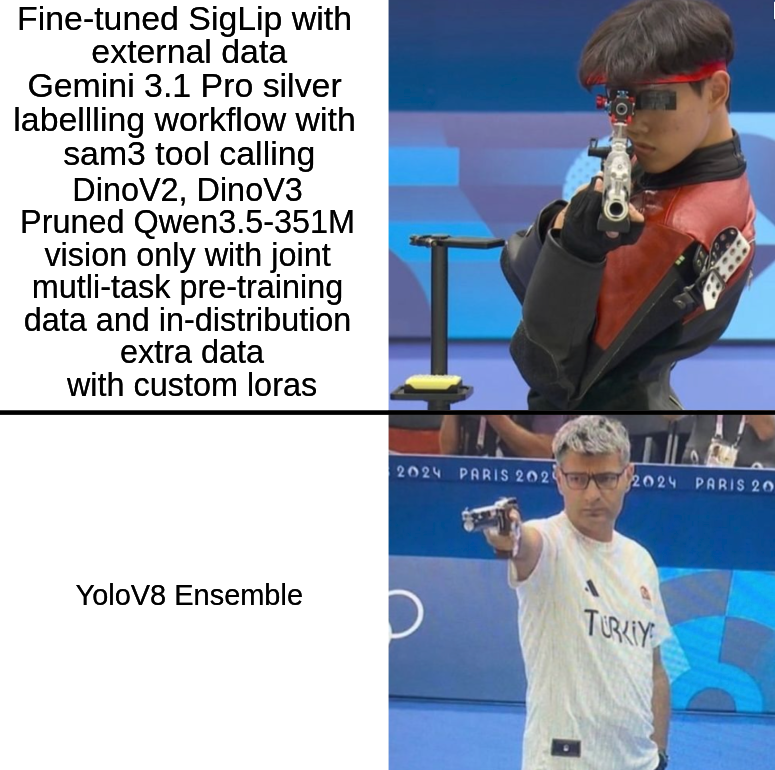
\includegraphics[width=0.55\textwidth]{memes/image.png}
\caption{The competition experience, summarized.
Many teams built sophisticated pipelines combining fine-tuned vision-language models, generative AI for synthetic data, and contrastive learning --- only to be outperformed by a well-configured YOLO ensemble trained on the provided data alone.
Meme credit: Markus Hei (NM i AI 2026 Slack).}
\label{fig:meme}
\end{figure}

% ===========================================================================
\section{Introduction}
\label{sec:intro}

NM i AI is Norway's national AI competition, held as a 69-hour event where teams compete across three independent challenges.
The 2026 edition ran March~19--22 with tasks in AI agents (Tripletex), prediction engines (Astar), and object detection (NorgesGruppen Data).
Teams' overall ranking is determined by normalized scores across all three tasks, though each task also has its own leaderboard.

Task~3 asked participants to build a product detection system for grocery store shelves.
Given a photograph of a store shelf section, the system must detect every visible product with a bounding box and classify it into one of 356 product categories.
The score combines detection and classification quality:
\begin{equation}
    \text{Score} = 0.7 \times \text{mAP}_{\text{det}}@0.5 + 0.3 \times \text{mAP}_{\text{cls}}@0.5
    \label{eq:score}
\end{equation}

Submissions ran on a sandboxed server with Python~3.11, PyTorch~2.6.0, Ultralytics~8.1.0, an NVIDIA~L4 GPU, a 300-second time limit, no network access, and a 420\,MB ZIP size cap.
Teams could submit at most three times per day.
Critically, the public leaderboard used during the competition was scored on a different test set from the final private ranking --- making generalization the decisive factor.

% ===========================================================================
\section{The Domain: Grocery Shelf Recognition}
\label{sec:domain}

Automated shelf recognition is a growing area of applied computer vision, driven by the retail industry's need for real-time inventory monitoring, planogram compliance checking, and out-of-stock detection.
NorgesGruppen, Norway's largest grocery retailer, provided the dataset for this challenge.
The most closely related public benchmark is SKU-110K~\cite{goldman2019sku110k}, a densely packed shelf detection dataset with 11,762 images.
Our task is harder in one key dimension (356 fine-grained classes vs.\ single-class detection) but easier in others (less dense, canonical orientations).

The domain has characteristics that distinguish it from standard object detection benchmarks.
Products are densely packed in regular grid-like arrangements, with heavy occlusion along shelf edges.
The visual differences between products are often subtle --- two coffee packages from the same brand may differ only in a ``100g'' vs.\ ``200g'' label, requiring near-OCR-level discrimination.
Products always appear in a canonical upright orientation (unlike general object detection where objects can appear at any angle), which creates opportunities for domain-specific augmentation choices.
The training set of 248 images is tiny by modern standards, making overfitting a constant threat.

Additionally, the competition provided studio-quality reference images of each product from multiple angles (front, back, sides, top, bottom).
Several teams attempted to leverage these for gallery-based classification or synthetic data generation, with mixed results discussed in Section~\ref{sec:community}.

% ===========================================================================
\section{The Generalization Problem}
\label{sec:generalization}

The central challenge was not building a good detector --- it was building one that generalizes.
With 248 training images across 356 categories, every design decision carried the risk of overfitting.
We identified three levels of generalization failure during the competition.

First, the \textbf{training-to-validation gap}.
A YOLOv8l model with seed~77 achieved val~mAP~0.804 but scored only 0.770 on the public test, while a YOLOv8x with lower val~mAP scored 0.780.
With roughly 37 validation images (15\% of 248), local metrics are simply too noisy to be reliable.

Second, the \textbf{local-to-public gap}.
Models trained with \texttt{cls=2.0} (double classification loss weight) scored +0.015 higher on training-set evaluation but showed zero improvement on the public test.
Classification-specialized models memorize training distributions rather than learning generalizable features.

Third, and most importantly, the \textbf{public-to-private gap}.
The final private test set differed from the public leaderboard.
Our submission moved from 4th on public to 1st on private, while competitors who had optimized for the public leaderboard dropped.
This confirmed our generalization-first strategy.

Our strategy was informed by studying winning solutions from related Kaggle competitions, particularly Global Wheat Detection~\cite{david2020globalwheat} (domain shift in test set, WBF ensembles), Great Barrier Reef~\cite{gbr2021} (dense detection with tiled training and WBF), VinBigData~\cite{vinbigdata2021} (low data, multi-architecture ensembles), and Sartorius~\cite{sartorius2021} (only 606 images, external pre-training critical).
The recurring pattern across winners was clear: ensembles with WBF, architecture diversity, and aggressive data utilization.

These observations produced three design principles that guided all subsequent decisions: train on the full dataset without a validation split; maximize architectural diversity so that models fail independently; and reject any technique that shows strong local improvement but no test-set gain.

% ===========================================================================
\section{Method}
\label{sec:method}

\subsection{Architecture Diversity}
\label{sec:diversity}

The core of our winning submission is a heterogeneous ensemble of three architectures, each contributing a different ``view'' of the data.

\begin{table}[H]
\centering
\caption{The three models in the winning ensemble.}
\label{tab:models}
\begin{tabular}{@{}llll@{}}
\toprule
\textbf{Model} & \textbf{Architecture} & \textbf{Training Strategy} & \textbf{Role} \\
\midrule
fulldata\_x & YOLOv8x (68.2M params) & Standard augmentation & Strong baseline \\
nf\_11x\_s42 & YOLO11x~\cite{ultralytics2024yolo11} (56.9M params) & No vertical flip & Different backbone \\
v8l\_highaug & YOLOv8l (43.7M params) & Heavy augmentation & Regularized complement \\
\bottomrule
\end{tabular}
\end{table}

The models differ along three orthogonal axes.
Architecturally, YOLOv8x and YOLO11x have different backbone structures and feature pyramid designs, producing genuinely different error patterns.
In terms of augmentation, the noflip model learns stronger vertical-orientation features while the heavy-augmentation model (mixup=0.3, copy-paste=0.3, rotation up to 10 degrees) learns more robust, regularized features.
In terms of capacity, the range from 43.7M to 68.2M parameters gives different bias-variance tradeoffs.

This three-axis diversity means the models fail on different products, and WBF can correct individual errors through fusion.
Homogeneous ensembles (3$\times$YOLOv8x with different seeds) share failure modes and benefit less from fusion.

\subsection{Training}
\label{sec:training}

All models were trained on the full 248-image training set without holding out a validation split.
We found early on that withholding even 15\% of data significantly hurts performance on this small dataset, and that the resulting validation metrics do not predict test performance.

Training used 150 epochs with cosine learning rate scheduling and AdamW optimization at 640$\times$640\,px input resolution.
Mosaic augmentation was enabled with close-mosaic at epoch~130.
All three models used seed~42 --- diversity comes from architecture and augmentation choices, not random seed variation.

The noflip model (\texttt{flipud=0.0}) deserves special mention.
Since grocery products are never upside-down on shelves, vertical flip augmentation creates unrealistic training examples.
Disabling it improved local classification scores by +0.008, and when combined with the YOLO11x architecture, contributed to the ensemble's generalization.

\subsection{FP16 ONNX Export}

The sandbox environment's PyTorch~2.6.0 breaks \texttt{.pt} model loading from Ultralytics due to a change in \texttt{torch.load()} defaults.
We exported all models to ONNX with FP16 quantization, which also halved model size with negligible accuracy loss ($<$0.001~mAP).
The three models total approximately 326\,MB (131 + 110 + 85\,MB), fitting within the 420\,MB submission limit.

\subsection{Multi-Scale Inference with TTA}

Products on grocery shelves span a wide range of scales, from large cereal boxes to small tea packets.
We run each model at both 640$\times$640\,px and 800$\times$800\,px, with horizontal-flip test-time augmentation at each scale.
This produces $3 \times 2 \times 2 = 12$ inference passes per image.
We tested 960\,px as a third scale but found diminishing returns ($-$0.001 on test).

\subsection{Weighted Boxes Fusion}

Rather than Non-Maximum Suppression, we use Weighted Boxes Fusion~\cite{solovyev2021wbf} to merge the 12 prediction sets.
WBF produces more accurate bounding box coordinates by weighted averaging of matched detections rather than discarding overlapping boxes.

The \texttt{absent\_model\_aware\_avg} confidence type is essential for our diverse ensemble.
It averages scores only across models that actually produced a matching detection ($N_{\text{present}}$), rather than dividing by the total number of models $M$.
This prevents the smaller YOLOv8l from dragging down confidence scores when it misses detections that the larger models catch.
We use $\text{iou\_thr} = 0.6$ and $\text{skip\_box\_thr} = 0.01$.

\subsection{Mathematical Formulation}

For completeness, we describe the key mathematical operations in the pipeline.

\paragraph{Letterbox preprocessing.}
Given an input image of size $(W_{\text{orig}}, H_{\text{orig}})$ and target size $S$, the letterbox transform computes a uniform scale factor $r = \min(S/W_{\text{orig}},\, S/H_{\text{orig}})$, resizes the image to $(W_{\text{new}}, H_{\text{new}}) = (\lfloor W_{\text{orig}} \cdot r \rfloor, \lfloor H_{\text{orig}} \cdot r \rfloor)$, and centers it on an $S \times S$ canvas with padding $(p_x, p_y)$.
Predicted coordinates are mapped back via $x_{\text{orig}} = (x_{\text{pred}} - p_x) / r$.

\paragraph{Weighted Boxes Fusion.}
Given $M$ models producing box sets $\{\mathcal{B}_1, \ldots, \mathcal{B}_M\}$, WBF clusters overlapping boxes with $\text{IoU} > \tau_{\text{wbf}}$ and computes the fused box as a confidence-weighted average:
\begin{equation}
    b_{\text{fused}} = \frac{\sum_{k=1}^{|C|} s_k \cdot b_k}{\sum_{k=1}^{|C|} s_k}
    \label{eq:wbf_box}
\end{equation}
The absent-model-aware fused score is:
\begin{equation}
    s_{\text{fused}} = \frac{\sum_{k=1}^{|C|} s_k}{N_{\text{present}}}
    \label{eq:absent_aware}
\end{equation}
where $N_{\text{present}} \leq M$ counts only models that contributed a box to cluster $C$.
Compare with the standard average $s_{\text{avg}} = \sum s_k / M$, which unfairly penalizes detections that only a subset of models find.

\paragraph{Mean Average Precision.}
For each class $c$, the Average Precision is the area under the precision-recall curve: $\text{AP}_c = \int_0^1 p_c(r)\, dr$.
A detection is a true positive if $\text{IoU} \geq 0.5$ with a ground-truth box of the same class.
The final metric is $\text{mAP}@0.5 = \frac{1}{|\mathcal{C}|} \sum_{c \in \mathcal{C}} \text{AP}_c$, weighted into the competition score via Equation~\ref{eq:score}.

% ===========================================================================
\section{Technique Radar}
\label{sec:radar}

Figure~\ref{fig:radar} provides a visual overview of all techniques explored during the competition.
The winning path runs through architecture diversity and multi-scale inference, while post-processing and specialization directions consistently showed diminishing or negative returns.

\begin{figure}[H]
\centering
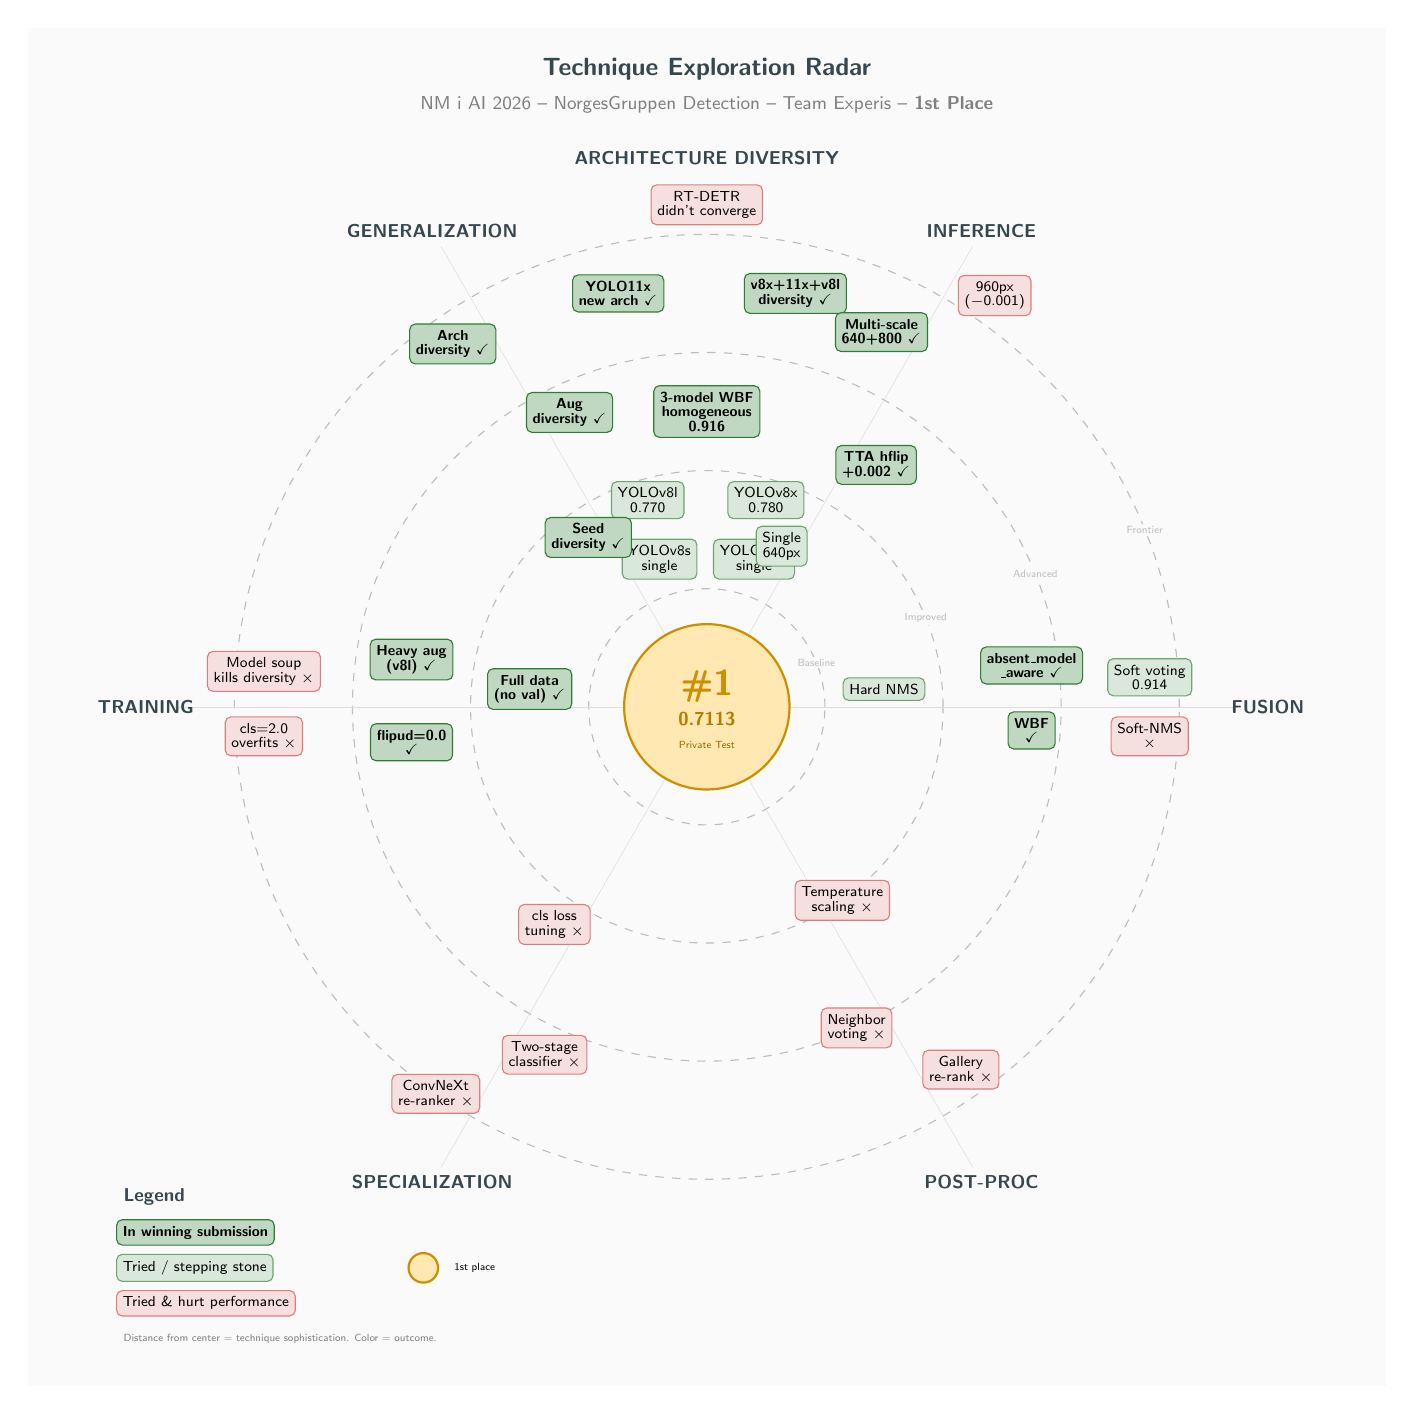
\begin{tikzpicture}[
    scale=0.75, transform shape,
    every node/.style={font=\sffamily},
    best/.style={fill=okgreen!30, draw=okgreen, rounded corners=2pt,
                 font=\sffamily\scriptsize\bfseries, inner sep=3pt, align=center},
    tried/.style={fill=okgreen!18, draw=okgreen!70, rounded corners=2pt,
                  font=\sffamily\scriptsize, inner sep=3pt, align=center},
    failed/.style={fill=failred!15, draw=failred!60, rounded corners=2pt,
                   font=\sffamily\scriptsize, inner sep=3pt, align=center},
    dirlbl/.style={font=\sffamily\small\bfseries, color=dirlabel},
]

\begin{scope}[on background layer]
  \fill[bgcream] (-11.5,-11.5) rectangle (11.5,11.5);
\end{scope}

\node[font=\sffamily\large\bfseries, color=dirlabel] at (0,10.8)
  {Technique Exploration Radar};
\node[font=\sffamily\small, color=black!50] at (0,10.2)
  {NM i AI 2026 -- NorgesGruppen Detection -- Team Experis -- \textbf{1st Place}};

\foreach \r/\lbl in {2/Baseline, 4/Improved, 6/Advanced, 8/Frontier}{
  \draw[ringgray, thin, dashed] (0,0) circle (\r);
  \node[font=\sffamily\tiny, color=ringgray, fill=bgcream, inner sep=1pt]
    at ({\r*cos(22)},{\r*sin(22)}) {\lbl};
}

\foreach \a in {0,60,...,300}{
  \draw[ringgray!50, very thin] (0,0) -- ({9*cos(\a)},{9*sin(\a)});
}

% Center - gold 1st place
\fill[goldcolor!30] (0,0) circle (1.4);
\draw[goldcolor!80!black, thick] (0,0) circle (1.4);
\node[font=\sffamily\LARGE\bfseries, color=goldcolor!80!black] at (0,0.35) {\#1};
\node[font=\sffamily\small\bfseries, color=goldcolor!70!black] at (0,-0.2) {0.7113};
\node[font=\sffamily\tiny, color=goldcolor!60!black] at (0,-0.65) {Private Test};

% NORTH: Architecture Diversity
\node[dirlbl] at (0,9.3) {ARCHITECTURE DIVERSITY};
\node[tried] at (-0.8, 2.5) {YOLOv8s\\[-1pt]\scriptsize single};
\node[tried] at (0.8, 2.5) {YOLOv8m\\[-1pt]\scriptsize single};
\node[tried] at (-1.0, 3.5) {YOLOv8l\\[-1pt]\scriptsize 0.770};
\node[tried] at (1.0, 3.5) {YOLOv8x\\[-1pt]\scriptsize 0.780};
\node[best] at (0, 5.0) {3-model WBF\\[-1pt]\scriptsize homogeneous\\[-1pt]\scriptsize 0.916};
\node[best] at (-1.5, 7.0) {YOLO11x\\[-1pt]\scriptsize new arch \checkmark};
\node[best] at (1.5, 7.0) {v8x+11x+v8l\\[-1pt]\scriptsize \textbf{diversity} \checkmark};
\node[failed] at (0, 8.5) {RT-DETR\\[-1pt]\scriptsize didn't converge};

% ENE: Inference
\node[dirlbl] at ({9.3*cos(60)},{9.3*sin(60)}) {INFERENCE};
\node[tried] at ({3*cos(65)},{3*sin(65)}) {Single\\[-1pt]\scriptsize 640px};
\node[best] at ({5*cos(55)},{5*sin(55)}) {TTA hflip\\[-1pt]\scriptsize +0.002 \checkmark};
\node[best] at ({7*cos(65)},{7*sin(65)}) {Multi-scale\\[-1pt]\scriptsize 640+800 \checkmark};
\node[failed] at ({8.5*cos(55)},{8.5*sin(55)}) {960px\\[-1pt]\scriptsize ($-$0.001)};

% EAST: Fusion
\node[dirlbl] at (9.5,0) {FUSION};
\node[tried] at (3, 0.3) {Hard NMS};
\node[best] at (5.5, -0.4) {WBF\\[-1pt]\scriptsize \checkmark};
\node[best] at (5.5, 0.7) {absent\_model\\[-1pt]\scriptsize \_aware \checkmark};
\node[failed] at (7.5, -0.5) {Soft-NMS\\[-1pt]\scriptsize $\times$};
\node[tried] at (7.5, 0.5) {Soft voting\\[-1pt]\scriptsize 0.914};

% SSE: Post-Processing
\node[dirlbl] at ({9.3*cos(-60)},{9.3*sin(-60)}) {POST-PROC};
\node[failed] at ({4*cos(-55)},{4*sin(-55)}) {Temperature\\[-1pt]\scriptsize scaling $\times$};
\node[failed] at ({6*cos(-65)},{6*sin(-65)}) {Neighbor\\[-1pt]\scriptsize voting $\times$};
\node[failed] at ({7.5*cos(-55)},{7.5*sin(-55)}) {Gallery\\[-1pt]\scriptsize re-rank $\times$};

% WEST: Training
\node[dirlbl] at (-9.5,0) {TRAINING};
\node[best] at (-3.0, 0.3) {Full data\\[-1pt]\scriptsize (no val) \checkmark};
\node[best] at (-5.0, -0.6) {flipud=0.0\\[-1pt]\scriptsize \checkmark};
\node[best] at (-5.0, 0.8) {Heavy aug\\[-1pt]\scriptsize (v8l) \checkmark};
\node[failed] at (-7.5, -0.5) {cls=2.0\\[-1pt]\scriptsize overfits $\times$};
\node[failed] at (-7.5, 0.6) {Model soup\\[-1pt]\scriptsize kills diversity $\times$};

% WSW: Specialization
\node[dirlbl] at ({9.3*cos(240)},{9.3*sin(240)}) {SPECIALIZATION};
\node[failed] at ({4.5*cos(235)},{4.5*sin(235)}) {cls loss\\[-1pt]\scriptsize tuning $\times$};
\node[failed] at ({6.5*cos(245)},{6.5*sin(245)}) {Two-stage\\[-1pt]\scriptsize classifier $\times$};
\node[failed] at ({8*cos(235)},{8*sin(235)}) {ConvNeXt\\[-1pt]\scriptsize re-ranker $\times$};

% NNW: Generalization
\node[dirlbl] at ({9.3*cos(120)},{9.3*sin(120)}) {GENERALIZATION};
\node[best] at ({3.5*cos(125)},{3.5*sin(125)}) {Seed\\[-1pt]\scriptsize diversity \checkmark};
\node[best] at ({5.5*cos(115)},{5.5*sin(115)}) {Aug\\[-1pt]\scriptsize diversity \checkmark};
\node[best] at ({7.5*cos(125)},{7.5*sin(125)}) {Arch\\[-1pt]\scriptsize diversity \checkmark};

% Legend
\begin{scope}[shift={(-10,-9.5)}]
  \node[font=\sffamily\small\bfseries, color=dirlabel, anchor=west] at (0,1.2) {Legend};
  \node[best, anchor=west] at (0, 0.6) {In winning submission};
  \node[tried, anchor=west] at (0, 0) {Tried / stepping stone};
  \node[failed, anchor=west] at (0, -0.6) {Tried \& hurt performance};
  \draw[goldcolor!80!black, thick, fill=goldcolor!30] (5.2,0) circle (0.25);
  \node[font=\sffamily\tiny, anchor=west] at (5.6,0) {1st place};
  \node[font=\sffamily\tiny, color=black!50, anchor=west] at (0,-1.2)
    {Distance from center = technique sophistication. Color = outcome.};
\end{scope}

\end{tikzpicture}
\caption{Technique exploration radar showing all approaches tried during the competition. The winning path runs through architecture diversity (North) and multi-scale inference (ENE). Post-processing and specialization (red nodes) consistently failed to generalize.}
\label{fig:radar}
\end{figure}

% ===========================================================================
\section{Experiments and Results}
\label{sec:results}

\subsection{Submission History}

Table~\ref{tab:submissions} shows all competition submissions.
The progression tells the story of our approach: the massive jump from single model to ensemble, followed by incremental gains from inference improvements and diversity.

\begin{table}[H]
\centering
\caption{Competition submissions with public test scores. The final submission achieved 0.9226 on public and 0.7113 on private test (1st place).}
\label{tab:submissions}
\small
\begin{tabular}{@{}clccc@{}}
\toprule
\textbf{\#} & \textbf{Submission} & \textbf{Public Test} & \textbf{$\Delta$} & \textbf{Key Change} \\
\midrule
1 & \texttt{yolov8x\_onnx\_clean}       & 0.7802 & ---     & Single model baseline \\
2 & \texttt{yolov8l\_640\_s77}           & 0.7700 & $-$0.010 & Architecture variant \\
3 & \texttt{onnx\_ensemble\_ms\_tuned}   & 0.9091 & $+$0.129 & WBF ensemble (x+m+s) \\
4 & \texttt{softvote\_3x\_fp16}          & 0.9142 & $+$0.005 & Soft class voting \\
5 & \texttt{wbf\_3x\_fp16\_tta}          & 0.9160 & $+$0.002 & WBF + TTA hflip \\
6 & \texttt{wbf\_2x1l\_multiscale\_tta}  & 0.9210 & $+$0.005 & Multi-scale + arch diversity \\
7 & \texttt{candidate11\_noflip\_l}      & 0.9215 & $+$0.001 & Training diversity \\
8 & \texttt{sub1\_triple\_arch}          & 0.9190 & $-$0.003 & YOLO11x first attempt \\
\rowcolor{okgreen!15}
9 & \texttt{sub2\_yolo11x\_swap}         & \textbf{0.9226} & $+$0.001 & \textbf{Architecture diversity (winner)} \\
\bottomrule
\end{tabular}
\end{table}

\subsection{Ablation}

Table~\ref{tab:ablation} isolates the contribution of each technique.
Ensembling provides the single largest gain, with multi-scale and architecture diversity contributing the final margin.

\begin{table}[H]
\centering
\caption{Ablation study on the public test set.}
\label{tab:ablation}
\begin{tabular}{@{}lcc@{}}
\toprule
\textbf{Configuration} & \textbf{Public Test} & \textbf{$\Delta$} \\
\midrule
Single YOLOv8x (640px)                            & 0.7802 & --- \\
$+$ WBF 3-model ensemble (same arch)              & 0.9091 & $+$0.1289 \\
$+$ TTA horizontal flip                           & 0.9160 & $+$0.0069 \\
$+$ Multi-scale (640+800px)                        & 0.9210 & $+$0.0050 \\
$+$ Architecture diversity (YOLO11x + YOLOv8l)    & 0.9226 & $+$0.0016 \\
\bottomrule
\end{tabular}
\end{table}

\subsection{What Did Not Generalize}

Table~\ref{tab:negative} documents approaches that improved local metrics but failed on test.
The most dangerous techniques were those with large local improvements --- they build false confidence and waste limited submission budget.

\begin{table}[H]
\centering
\caption{Techniques that failed to generalize.}
\label{tab:negative}
\small
\begin{tabular}{@{}lccc@{}}
\toprule
\textbf{Technique} & \textbf{Local $\Delta$} & \textbf{Test $\Delta$} & \textbf{Why it failed} \\
\midrule
cls=2.0 loss weight          & $+$0.015 & $+$0.000 & Memorizes training classes \\
Two-stage classifier         & $+$0.007 & $-$0.011 & 96.9\% train acc, overfits to crops \\
Gallery re-ranking           & $+$0.000 & $-$0.003 & Can't distinguish fine-grained variants \\
Model soup (weight avg)      & $-$0.015 & N/A      & Destroys diversity for ensembles \\
Neighbor class voting        & $-$0.004 & N/A      & Flips correct predictions \\
960px third scale            & N/A      & $-$0.001 & Diminishing returns \\
\bottomrule
\end{tabular}
\end{table}

% ===========================================================================
\section{Tooling and Infrastructure}
\label{sec:tooling}

\subsection{Training Infrastructure}

All model training ran on Azure Machine Learning, using up to 8 nodes of Standard\_NC4as\_T4\_v3 (NVIDIA T4, 16\,GB VRAM each), generously provided by Experis.
Over 69 hours we executed 150+ training runs spanning 7 architectures (YOLOv8x/l/m/s, YOLO11x, RT-DETR, YOLO26x), 14 random seeds, and numerous augmentation configurations.
Job definitions were managed as YAML files, enabling rapid experiment dispatch.

In hindsight, we should also have leveraged the free GCP GPU credits provided to all competition teams by the organizers.
We used GCP for the other two tasks but not for this one, which limited our parallel training throughput during the critical final hours.

\subsection{Analytics Dashboard}

We built a Streamlit-based analytics dashboard that provided real-time visibility into our experiment results.
The dashboard tracked all training runs from \texttt{experiments.csv}, displayed detection versus classification mAP breakdowns from local evaluations, and most importantly identified which product categories each model struggled with.

This per-category failure analysis directly informed our architecture diversity strategy.
By comparing confusion matrices across models, we could see that YOLOv8x and YOLO11x failed on \emph{different} product pairs --- confirming that combining them would produce complementary predictions rather than correlated errors.

\subsection{Prediction Caching}

To enable rapid post-processing sweeps, we cached each model's raw detections (boxes, scores, full 356-dim class probability vectors) on all 248 training images.
This allowed testing all $\binom{6}{3} = 20$ three-model combinations from 6 candidate models in under 60 seconds, and sweeping 21 WBF parameter configurations in under 30 seconds --- compared to 60+ minutes for a single full inference run.

\subsection{Submission Validation}

After an early \texttt{import sys} statement in a submission caused an automatic sandbox ban (the security scanner immediately blocks any submission containing prohibited imports), we built a comprehensive validation pipeline.
A dedicated \texttt{validate\_submission.py} script checks all sandbox rules: 23 blocked import modules, blocked function calls, file count and size limits, the 3-weight-file maximum, path traversal, binary executables, and output format compliance.
A Pytest suite runs 10 automated tests per ZIP before every build, and a Docker-based local sandbox replica provides end-to-end validation.
This pipeline prevented at least two additional invalid submissions.

% ===========================================================================
\section{Community Approaches}
\label{sec:community}

Post-competition discussion in the official Slack channel revealed interesting patterns across teams.
What follows is a summary of approaches shared by participants, contrasted with our own.

\paragraph{Synthetic data was widely attempted but rarely helped.}
Andr\'e Mikalsen (0.920) used Nano Banana~2 to generate variations of product images showing them from different angles, lying down, and in shelf shadows --- the most creative synthetic data approach reported.
Andreas Hatlem (0.9220) generated approximately 1,400 synthetic images by pasting product reference photos onto shelf backgrounds with alpha blending and random transformations, but found models trained on this data plateaued at 0.788 versus 0.799 without it.
Markus Hei went further, physically visiting stores to photograph shelves of underrepresented products and using Gemini with SAM3 for silver labeling --- but his best score remained the YOLOv8 baseline from day~1.
Dag Koding from DKIT also tried synthetic data and got worse results, and even considered creating 3D models of product packaging but ran out of time.
Ludvig {\O}vrevik used Nano Banana to create empty shelf images and placed products on them, producing 3,000 synthetic images that ultimately did not improve his model.

Our approach stands out by its absence of synthetic data.
We focused entirely on the 248 provided shelf images, investing our time in model architecture diversity and inference strategy rather than data augmentation.
The domain gap between clean product photos and real shelf crops proved too large for most synthetic approaches to bridge.

\paragraph{Multi-model ensembles were the universal winning strategy.}
Andreas Hatlem (0.9220) used 3-model WBF with YOLOv8x + YOLO26-x + a K-fold model at 1280px, and independently discovered the same diversity principle we relied on: his weakest individual model (K-fold~2, 0.749~mAP) consistently gave the best ensemble results, and every swap for a stronger model made the ensemble worse.
Walgermo from Matriks (0.9208) used a 3-model YOLOv8l ensemble with random seeds after a parameter sweep.

\paragraph{Training on all 248 images was a recurring finding.}
Multiple teams, including Hatlem and ourselves, found that withholding images for validation hurt performance more than the validation signal was worth.
Mikalsen generated synthetic validation images and used Gemini~3.1 Flash for classification labels instead --- a creative workaround for the same problem.

\paragraph{Post-processing tuning universally failed.}
Hatlem reported that ``every single tweak hurt the score'' for post-processing (WBF parameters, Soft-NMS, temperature scaling, multi-scale TTA variants), matching our own experience exactly.

\paragraph{The unknown product ambiguity.}
P{\aa}l Bentsen raised an interesting question about the task specification: should products present in the image but not belonging to any of the 356 annotated categories be detected and classified as an ``unknown product'' class, or should they be ignored entirely?
As shown in Figure~\ref{fig:unknown}, the Natreen sweetener products on the shelf have no ground truth annotations despite being clearly visible products.
In a real-world retail system, detecting all products (including unknown ones) would be essential for inventory management.
The competition's handling of this edge case was ambiguous --- and the answer affected model design, since detecting extra products that the evaluator ignores would generate false positives that hurt the score.

\begin{figure}[H]
\centering
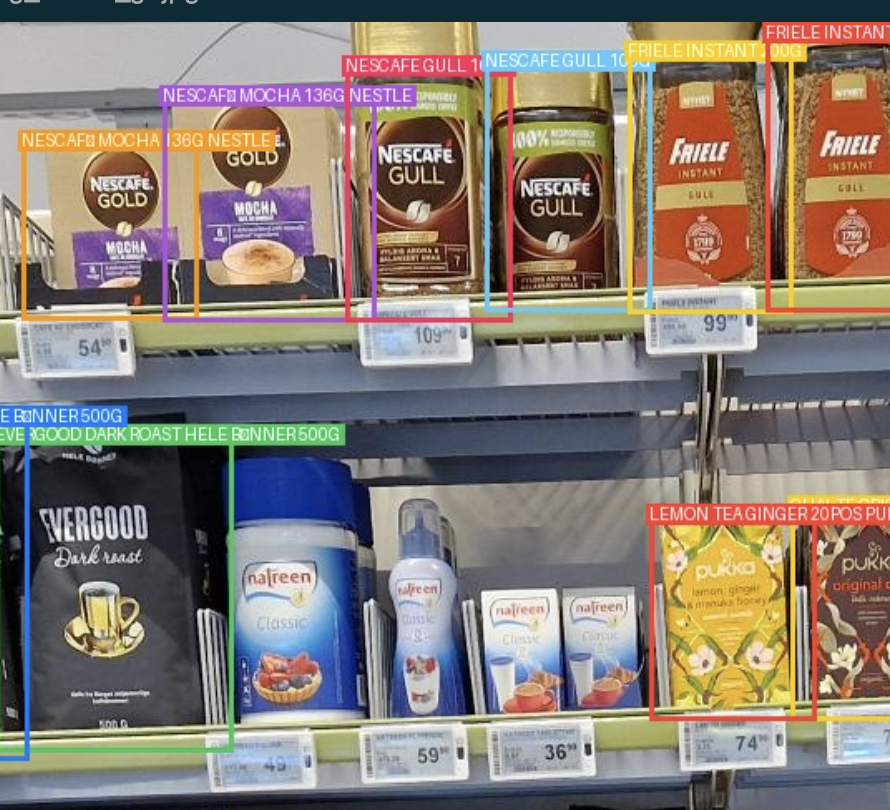
\includegraphics[width=0.85\textwidth]{memes/unknown_product.png}
\caption{The unknown product problem, highlighted by P{\aa}l Bentsen.
The Natreen products on the lower shelf have no ground truth annotations.
Should a detection system ignore them, or classify them as ``unknown''?
The competition did not clearly specify this, creating a design dilemma for participants.}
\label{fig:unknown}
\end{figure}

\paragraph{Annotation quality was questioned.}
P{\aa}l Bentsen also observed that the ground truth annotations contained outright errors, with their model making correct predictions that lacked corresponding annotations.
They manually corrected a selection and retrained from scratch, gambling that the private test set would be better annotated.

\subsection{Why Synthetic Data Failed}
\label{sec:synthetic}

The community results paint a clear picture: at least six teams tried synthetic data generation, and none achieved improvements.
We believe several factors explain this.

First, the \textbf{domain gap} between product reference images (clean studio shots on white backgrounds) and real shelf crops (complex lighting, reflections, partial occlusion, price tags, shelf edges) is substantial.
Simple compositing techniques (alpha blending, pasting onto backgrounds) do not capture the visual complexity of how products actually appear on shelves.

Second, the \textbf{evaluation metric penalizes noise}.
Even if synthetic data helps the model detect more products, any systematic bias it introduces (wrong scale, unrealistic shadows, incorrect spatial relationships between products) creates false positives or classification errors that directly reduce mAP.

Third, the \textbf{dataset is already highly specialized}.
The 248 real shelf images contain approximately 22,700 annotations of actual products in their real retail context.
The signal-to-noise ratio of these real annotations is far higher than any synthetic generation pipeline could achieve in the 69-hour time constraint.

Fourth, and most subtly, synthetic data may \textbf{reduce ensemble diversity}.
If all models in an ensemble are trained on the same synthetic data, they learn the same synthetic artifacts and fail on the same real-world edge cases.
Our approach of using only real data but varying the augmentation strategy and architecture preserved the independent failure modes that WBF exploits.

% ===========================================================================
\section{Lessons Learned}
\label{sec:lessons}

\textbf{Generalization beats optimization.}
Our most important lesson is that optimizing for known test sets is a losing strategy when the final evaluation uses a different distribution.
We moved from 4th on the public leaderboard to 1st on the private test.
Teams that achieved higher public scores by fine-tuning their approach dropped in the final ranking.

\textbf{Diversity over specialization.}
Every attempt at specialization (classification loss tuning, two-stage classifiers, gallery re-ranking, model soups) failed to generalize.
Every form of diversity (architecture, augmentation, scale) helped.
On small datasets, invest in making \emph{different types of predictions} rather than \emph{better predictions of the same type}.

\textbf{Reject locally-good changes.}
The hardest discipline was rejecting techniques that showed clear local improvements.
A model with \texttt{cls=2.0} scored +0.015 higher locally --- a massive improvement by any measure.
But it showed zero test improvement.
The courage to walk away from validated-but-not-generalizing improvements was the single most important factor in our win.

\textbf{The domain matters.}
Grocery shelf recognition has strong structural priors (upright products, grid layouts, canonical lighting) that reward domain-aware choices like disabling vertical flip augmentation.
But it also has adversarial properties (near-identical products differing only in small text) that defeat standard feature extractors.
Understanding both aspects shaped our approach.

% ===========================================================================
\section{Conclusion}
\label{sec:conclusion}

We presented the winning solution to the NM i AI 2026 NorgesGruppen product detection task, achieving 1st place with 0.7113~mAP on the private test set.
Our approach combined three YOLO architectures (YOLOv8x, YOLO11x, YOLOv8l) with diverse augmentation strategies, multi-scale inference, and Weighted Boxes Fusion --- without any synthetic data, external datasets, or post-processing tricks.
The primary lesson for practitioners: when the test distribution is uncertain, bet on diversity, not accuracy.

\subsection*{Acknowledgments}

We thank \textbf{Experis} for providing the Azure ML compute resources that enabled our 150+ training runs --- without dedicated GPU access, the scale of experimentation described here would not have been possible.
We also thank the NM i AI organizers at \textbf{Astar Technologies} for running an excellent competition, \textbf{NorgesGruppen Data} for providing a genuinely challenging and well-crafted task, and all the participants whose creative approaches (documented in Section~\ref{sec:community}) made the post-competition discussion as educational as the competition itself.
We note that free GCP GPU credits were provided to all teams by the organizers; we used these for Tasks~1 and~2 but not for this task, which in hindsight was a missed opportunity for additional training throughput.

% ===========================================================================
\bibliographystyle{plain}
\begin{thebibliography}{99}

\bibitem[Jocher et~al.(2023)]{jocher2023yolov8}
G.~Jocher, A.~Chaurasia, and J.~Qiu.
\newblock Ultralytics {YOLO}, 2023.
\newblock \url{https://github.com/ultralytics/ultralytics}.

\bibitem[Solovyev et~al.(2021)]{solovyev2021wbf}
R.~Solovyev, W.~Wang, and T.~Gabruseva.
\newblock Weighted boxes fusion: Ensembling boxes from different object detection models.
\newblock \emph{Image and Vision Computing}, 107:104117, 2021.

\bibitem[Lin et~al.(2014)]{lin2014coco}
T.-Y.~Lin, M.~Maire, S.~Belongie, J.~Hays, P.~Perona, D.~Ramanan, P.~Doll{\'a}r, and C.~L.~Zitnick.
\newblock Microsoft {COCO}: Common objects in context.
\newblock In \emph{ECCV}, 2014.

\bibitem[Goldman et~al.(2019)]{goldman2019sku110k}
E.~Goldman, R.~Herzig, A.~Eisenschtat, J.~Goldberger, and T.~Hassner.
\newblock Precise detection in densely packed scenes.
\newblock In \emph{CVPR}, 2019.
\newblock Dataset: \url{https://docs.ultralytics.com/datasets/detect/sku-110k/}.

\bibitem[David et~al.(2020)]{david2020globalwheat}
E.~David, S.~Madec, P.~Sadeghi-Tehran, et~al.
\newblock Global wheat head detection ({GWHD}) dataset.
\newblock \emph{Plant Phenomics}, 2020.
\newblock Kaggle: \url{https://www.kaggle.com/competitions/global-wheat-detection}.

\bibitem[GBR 2021]{gbr2021}
Kaggle.
\newblock {TensorFlow} --- Great Barrier Reef.
\newblock \url{https://www.kaggle.com/competitions/tensorflow-great-barrier-reef}, 2021.
\newblock 1st place: 6-model YOLOv5 ensemble with tiled training and WBF.

\bibitem[VinBigData 2021]{vinbigdata2021}
Kaggle.
\newblock {VinBigData} Chest X-ray Abnormalities Detection.
\newblock \url{https://www.kaggle.com/competitions/vinbigdata-chest-xray-abnormalities-detection}, 2021.
\newblock 1st place: YOLOv5 + EfficientDet ensemble with WBF, 15K images, 14 classes.

\bibitem[Sartorius 2021]{sartorius2021}
Kaggle.
\newblock Sartorius Cell Instance Segmentation.
\newblock \url{https://www.kaggle.com/competitions/sartorius-cell-instance-segmentation}, 2021.
\newblock 606 images only; winner used external pre-training on LIVECell.

\bibitem[Ultralytics(2024)]{ultralytics2024yolo11}
Ultralytics.
\newblock {YOLO11}: Next-generation real-time object detection, 2024.
\newblock \url{https://docs.ultralytics.com/models/yolo11/}.

\end{thebibliography}

\end{document}
